\chapter{Introduction}
 \section{Introduction}


Database Management System (DBMS) has thrived since its first appearance and it remains the dominant manner for storing various kinds of information. Specifically, DBMSs have been extensively used in many fields and have applications in almost all companies as they provide a relatively easy way of performing various operations on data, such as insertion, deletion and modification[4,6,7]. For that reason, applications can be implemented efficiently and reliably without the need for handling low-level issues such as concurrent and efficient access of data which it is taken cared by DBMS. Hence, the main role of a DBMS is not only to store data but also to provide a common interface for manipulating data. Figure 1.1 shows from a high-level point of view the structure of a modern DBMS.

In fact, in its early stage, each database system had its own interface and as a result migrating your SQL code among analogous systems it was almost impossible. Thus, all the code should be written again according to the specific DBMS interface. Nevertheless, as these systems were promising from their first appearance, a standardised language was unavoidable. Structured Query language (SQL) has become a standardised programming language for querying and managing data and has rapidly become the most widely used DBMS language[1].  Since then, comparable languages have been emerged over the years, SQL has persisted to be the dominant language since it has been easy to learn. In contrast with programming languages, where each language has its own benefits and usage, with SQL users and programmers can take advantage of it in order to learn a new language that it will be used by essentially all modern DBMSs and write SQL code that with minor changes it can be executed on any system. 

Moreover, the relational model (RM) is the mainstream model for the DBMSs for managing data and it is by far the most popular model for current DBMSs. It was proposed by Edgar F.Codd in 1969 [15,16] and it has brought a revolution in the area of data management due to its simplicity. A database that uses the relational model is known as a relational database. According to the relational model, data is stored in a database as tables and each table is composed of rows and columns. Also, each row of a table is known as a tuple based on RM and each column as characteristic or attribute. 

 \begin{figure} 
      \centering
      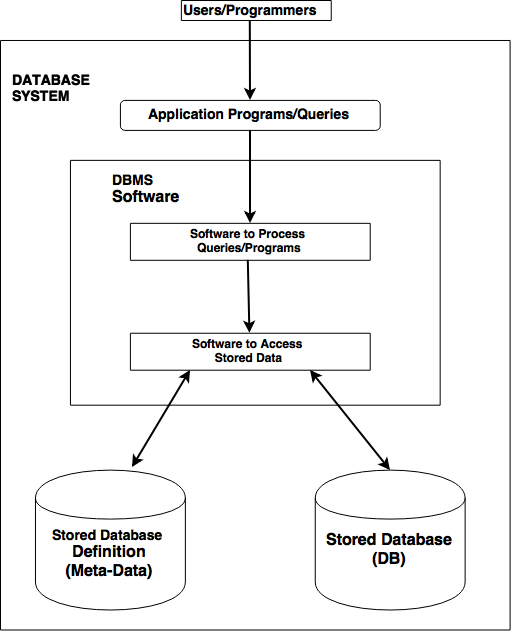
\includegraphics[width=\textwidth,height=6cm]{Images/db_arch}
      \caption{Abstract DBMS architecture}
      \label{fig:counting-methods}
    \end{figure}

  

 \section{Motivation}
 The SQL Standard is established a long time ago, and aims to provide a common interface among modern DBMSs. As each vendor implements its own DBMS, the extend of which this implementation complies with the SQL Standard is essential and needs to be studied. Database Systems have been evolved rapidly, and new features have been continuously added. As a result, users, programmers and companies that make use of such systems are facing enormous problems when it comes to migrating their existing SQL code in another DBMS as most of the times the SQL code is not completely portable. Mainly three major reasons are involved in the aforesaid problem.  Firstly, DBMS vendors do not always comply immediately to the latest SQL Standard because they have to cope with many considerations such as performance issues and better system management or even sometimes it is not practical to implement the entire Standard. Therefore vendors usually adopted new changes of the updated Standard into their next product releases. Secondly, DBMS vendors offer their own feature in order to be distinctive among other DBMSs which make SQL code less portable. Thirdly, the Standard is written in a natural language which makes the process of interpreting all the aspect of it in exactly the same way by all vendors, almost impossible.  Currently, there is no well-known architecture that can be used to test the SQL-Compliance among these systems and detect any incompatibility. Hence, this research aims to build a complete architecture for systematically discovering and highlighting both existing and new differences that may arise between any DBMSs. Afterwards, experimental evidences with a comprehensive explanation with respects to the SQL standard are provided. The experimental evidences will be significant for vendors of such systems, users, and companies that utilize these systems. Unfortunately, DBMSs do not always provide a meaningful message whenever an SQL code has a syntax error. As a consequence, it can take considerable time to detect and resolve any issue. By conducting this research, it is also intended to disclose all the incompatibilities that may exist and highlight all the differences, with such a way that it will make users and programmers aware about the current problems.


\section{Related Work }
As DBMSs are necessary for many fields some work has been conducted for implementing the standard of the SQL language. In fact, some parts of the Standard is interpreted differently and SQL code is not portable among these systems. Albeit, some notorious differences are demonstrated [1, 19], there is no well-known tool for evaluating these systems for identify differences. As a matter of fact, queries that executed without raising any error but interpreted differently by DBMSs can cause different result but without a tool to check the result is almost impossible to be exposed.  As a result, the current studies show results which have been detected by working with these systems. Having a tool for regularly checking the systems is imperative. 
 
 \section{Thesis Structure}

 The structure of the remainder of this thesis report is organized as follow:
 \begin{description}
   \item[$\bullet$ Chapter 2] introduces SQL language, SQL standards, the core commands of SQL and briefly describes the usage of the most important commands, and, afterwards it is introduced the main issues by illustrates problematic SQL queries. 
   
	\item[$\bullet$ Chapter 3] describes the main methodology for this research and briefly describes the explanation about the architecture which is implemented for systematically checking the SQL-compliance of current DBMSs.
   
   \item[$\bullet$ Chapter 4] provides a detailed explanation about the complete architecture and an explanation for each tool that composed the architecture is given. Also, it is discussed briefly the main issues that  are  addressed.

  \item[$\bullet$ Chapter 5] illustrates the main findings and provides an explanation about differences between current DBMSs with appropriate reference to the SQL standard. 

  \item[$\bullet$ Chapter 6] concludes this research project with explanation of what it is been achieved, and a summarize table of all the differences is provided. Afterwards,  they are provided futures ideas and extensions.  

   
\end{description} 

 
 
